\documentclass{beamer}

\usepackage[utf8]{inputenc}
\usepackage[slovene]{babel}
\usepackage{default}
\usepackage{graphicx}


\begin{document}
\title{Modeliranje \v sirjenja svetlobe vzdol\v z ograjenih teko\v cekristalnih defektnih linij}
\author{\begin{tabular}{rl}Avtor & Miha \v Can\v cula \\ Mentor & prof. dr. Slobodan \v Zumer \\ Somentor & doc. dr. Miha Ravnik\end{tabular}}
\date{3. september 2013}

\begin{frame}
 \titlepage
\end{frame}

\begin{frame}{Teko"ci kristali}
 \begin{columns}[t]
  \column{.5\textwidth}
  
  \begin{block}{Teko"ci kristali}
   \begin{itemize}
    \item Lastnosti teko"cin in kristalov
    \item Orientacijski red
    \item Delni pozicijski red
   \end{itemize}
  \end{block}
  
  \begin{block}{Opti"cne lastnosti}
   \begin{itemize}
    \item Dvolomnost
    \item Nadzor z zunanjimi polji
   \end{itemize}
  \end{block}

  \column[T]{.5\textwidth}
    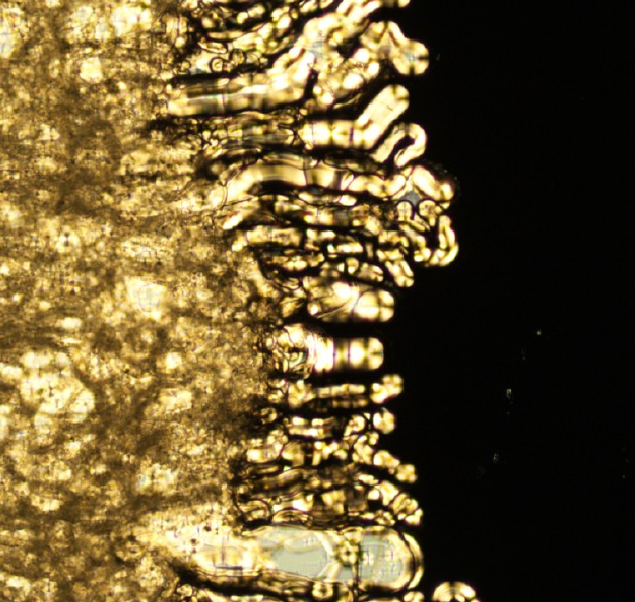
\includegraphics[width=\textwidth]{./Slike/tvorjenje2}
    
  \end{columns}
\end{frame}



\end{document}
